\documentclass[tikz,border=5pt]{standalone}
\usepackage{pgfplots}
\pgfplotsset{compat=1.18}
\usepackage{amsmath}
\usepackage{xcolor}
\usetikzlibrary{patterns}
\usepgfplotslibrary{fillbetween}

\begin{document}
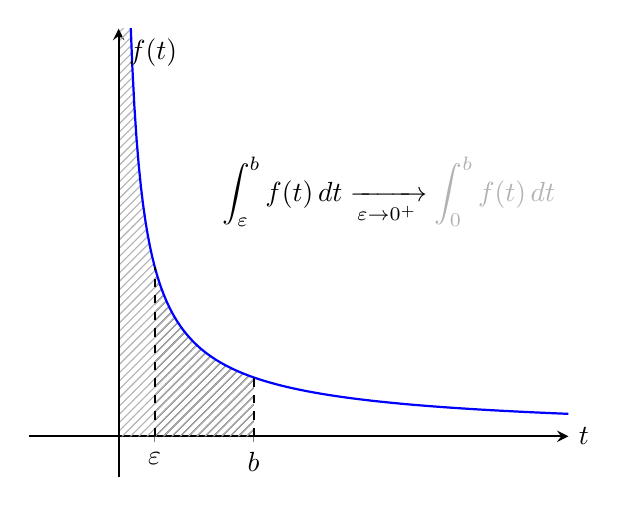
\begin{tikzpicture}
\begin{axis}[
    xmin=-1, xmax=5,
    ymin=-0.5, ymax=5,
    axis lines=middle,
    xlabel={$t$},   
    xlabel style={at={(axis cs:5,0)}, anchor=west},
    ylabel = $f(t)$,
    domain=0.1:5,
    samples=200,
    thick,
    xtick = {0.4,1.5},
    xticklabels = {$\varepsilon$,$b$},
    ytick=\empty,
]

% Aire hachurée sous f(t) entre \varepsilon et a
\addplot[domain=0.4:1.5, samples=100, pattern=north east lines,
         pattern color=black, draw=none, forget plot] {1/x^0.8} \closedcycle;

% Aire hachurée sous f(t) entre 0 et a (noir)
\addplot[domain=0:1.5, samples=100, pattern=north east lines,
         pattern color=gray!60, draw=none, forget plot] {1/x^0.8} \closedcycle;


% Courbe de t -> 1/\sqrt{t}
\addplot[blue, thick] {1/x^0.8};

% Repères verticaux
\draw[dashed] (axis cs:0.4,0) -- (axis cs:0.4,{1/0.4^0.8});
\draw[dashed] (axis cs:1.5,0) -- (axis cs:1.5,{1/1.5^0.8});

% Labels
\node at (axis cs:3.0,3) {$\displaystyle{\color{black}\int_\varepsilon^b f(t)\,dt} \xrightarrow[\varepsilon\to 0^+]{} {\color{gray!60}\int_0^{b} f(t)\,dt}$};
\end{axis}
\end{tikzpicture}
\end{document}
